\documentclass[12pt]{article}

% set margins and spacing
\addtolength{\textwidth}{1.3in}
\addtolength{\oddsidemargin}{-.65in} %left margin
\addtolength{\evensidemargin}{-.65in}
\setlength{\textheight}{9in}
\setlength{\topmargin}{-.5in}
\setlength{\headheight}{0.0in}
\setlength{\footskip}{.375in}
\renewcommand{\baselinestretch}{1.0}
\linespread{1.0}

% load miscellaneo`us packages
\usepackage{csquotes}
\usepackage[american]{babel}
\usepackage[usenames,dvipsnames]{color}
\usepackage{graphicx,amsbsy,amssymb, amsmath, amsthm, MnSymbol,bbding,times, verbatim,bm,pifont,pdfsync,setspace,natbib}

% enable hyperlinks and table of contents
\usepackage[pdftex,
bookmarks=true,
bookmarksnumbered=false,
pdfview=fitH,
bookmarksopen=true,hyperfootnotes=false]{hyperref}

% define environments
\newtheorem{definition}{Definition}
\newtheorem{fact}{Fact}
\newtheorem{result}{Result}
\newtheorem{proposition}{Proposition}



\begin{document}
\title{Development: The link between Manufacturing Employment and GDP in Developed and Developing Countries}
\author{Filippo Donà\thanks{Syracuse University, Economics Department. Email: kbuzard@syr.edu.} \and Lucia Rios-Luy\thanks{abc} \and Meghavarshini Iska \thanks{Syracuse University, Economics Student. Email: Meiska@syr.edu}}
\date{\vskip-.1in \today}
\maketitle

\vskip.3in
\begin{center} {\bf Abstract} \end{center}

\begin{quote}
{\small We examine the link between GDP growth and manufacturing employment, hypothesizing that there is a negative relationship between manufacturing employment and GDP; As manufacturing employment decreases, GDP increases. We source statistics
from Our World in Data charts, which examine these variables in all countries around the globe.
We create a distinction between developing and developed countries, setting the threshold at USD 20.000 Annual GDP per capita. We conduct a correlation test to compare these variables across both economies. 
The research conducted supports the hypothesis that manufacturing plays a more significant role in driving economic growth in developing countries compared to developed ones. The positive correlation in developing countries underscores the critical role of industrialization in early stages of economic
growth. In contrast, the negative correlation in developed countries highlights the global transition.}
\end{quote}

\bigskip

\section{Introduction} \label{sec:introduction}

Economic growth and development are two key terms in macroeconomics that have been studied by many, and it is vital to closely monitor and understand them to actualize and compose policies that drive development and growth in developing and developed countries. Our study examines the link between GDP growth and manufacturing employment. 

Moreover, when executing our analysis of the data, we observed that the correlation is different in developed and developing countries. In developed countries, we can see a negative corelation, while a positive correlation exists within developing countries. As manufacturing employment decreases, GDP increases in developed regions, and as manufacturing employment increases, so does GDP per capita in developing countries.

Our study hypothesizes that as GDP increases, there is a visible decrease in manufacturing employment, indicating a negative relationship between manufacturing employment and GDP. To reject our null hypothesis, we conducted a correlation test to compare our variables, GDP and manufacturing employment, across developing and developed countries. 
gituhub 

\textbf{Give a "road map" of the paper. Where will the reader find the various parts of your work?} (required)


\section{Literature Review} \label{sec:literature}


% Discuss at least five papers that are closely related to your results (more is better). Explain how they're related. Did you find something similar, or different? Did you look at a different context? Different time period? Different level of detail?

Industrialization continues to be a critical driver of economic growth and development, but manufacturing has increasingly become concentrated in some countries. The Industrial Revolution, which began in Britain around the late 18th century, catalyzed this economic shift, with nations like Britain leading in technological advancements and rising per capita incomes by the early 19th century (Allen, 2009). However, in the 21st century, manufacturing sectors have become concentrated in specific regions, with developing nations like those in Africa and parts of Asia still struggling to catch up (Rodrik, 2016). Despite these disparities, the overall significance of industrialization has not diminished, but its unequal distribution continues to contribute to income gaps that emerged as early as the mid-19th century (Pomeranz, 2000).

\section{Theoretical Analysis}
\label{sec:theory}
%Optional–may include in intro if it’s short.
This paper examines how manufacturing employment has affected growth development over time and place. Explicitly, we look at how the manufacturing employment sector will impact the gross domestic product per capita (GDP per capita) in developed and developing countries. Within our data analysis, we have observed that the correlation is different in developed and developing countries. In contrast, in developed countries, we can see a negative and positive correlation within developing countries. As manufacturing employment decreases, GDP increases in developed regions, and as manufacturing employment increases, so does GDP per capita in developing countries. This idea stems from the economic transformation seen in advanced nations, where progress in technology and the rise of service-based industries have reduced reliance on manufacturing labor yet continued to fuel GDP expansion. Using automation and innovation, developed economies achieve greater productivity with a smaller manufacturing workforce. In contrast, developing nations with lower GDP per capita base their growth on using natural resources and a heavy dependence on agricultural growth. In addition, they have a great potential for manufacturing employment, as they have a high low-wage labor market. This theoretical perspective forms the basis for our empirical investigation into the relationship between manufacturing employment and economic growth in different stages of development.


\section{Data}
\label{sec:data}

The Our World in Data chart dataset provides a comprehensive overview of various world indicators that estimate the position of each country's economy and development trajectory. This dataset has been sourced from the United Nations and multiple surveys covering social, economic, and environmental indicators for nearly all countries from 1990 to the present day. Each data point helps illustrate how manufacturing employment and GDP have changed over the years, using indicators for each country. For this analysis, we focused on two variables: \textit{``Manufacturing jobs as a share of total employment''} and \textit{``GDP per Capita,''} and categorized countries as developing or developed to observe the effects of manufacturing employment on growth rates.

\subsection{Data Scope and Definitions}
To ensure a clear comparison, we defined developed countries as those with a GDP per Capita equal to or greater than 20,000 USD and developing countries as those below this threshold. Additionally, we limited our analysis to data from 1990 to 2019 to avoid distortions caused by the COVID-19 pandemic.

\subsection{Summary Statistics}
To provide an overview of the dataset, we calculated descriptive statistics for each group of countries. These statistics, shown in Table~\ref{tab:summary-stats}, include the mean, median, and standard deviation for \textit{Manufacturing Employment Share} and \textit{GDP per Capita}.

\begin{table}[h!]
    \centering
    \caption{Summary Statistics for Developing and Developed Countries}
    \label{tab:summary-stats}
    \begin{tabular}{lccc}
        \hline
        \textbf{Variable} & \textbf{Mean} & \textbf{Median} & \textbf{Standard Deviation} \\
        \hline
        \textbf{Developing Countries} & & & \\
        Manufacturing Employment Share (\%) & 10.55 & 10.12 & 4.88 \\
        GDP per Capita (USD) & 17,957.71 & 13,500.00 & 20,173.73 \\
        \hline
        \textbf{Developed Countries} & & & \\
        Manufacturing Employment Share (\%) & 14.38 & 14.20 & 5.88 \\
        GDP per Capita (USD) & 36,008.51 & 34,200.00 & 21,577.48 \\
        \hline
    \end{tabular}
\end{table}

The summary statistics indicate clear differences between developing and developed countries. Developing countries show lower mean and median values for manufacturing employment share and GDP per capita, with higher variability in GDP per capita, reflecting significant economic disparity. Developed countries, on the other hand, exhibit higher means and medians with more stability in GDP per capita, highlighting advanced industrial structures.

\subsection{Graphical Trends}

\textbf{Developing countries:} 
\begin{figure}
    \centering
    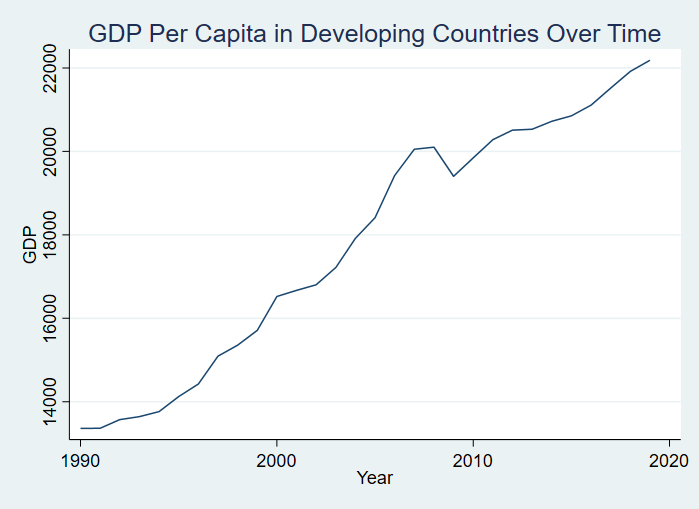
\includegraphics[width=0.5\linewidth]{GDP DEVELOPING GRAPH.png}
    \caption{Enter Caption}
    \label{fig:enter-label}
\end{figure}
\begin{figure}
    \centering
    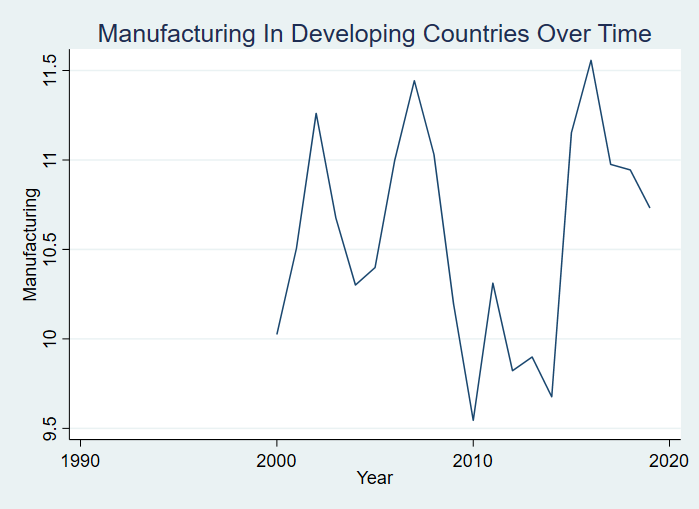
\includegraphics[width=0.5\linewidth]{FINAL GRAPH MFT DEVELOPING.png}
    \caption{Enter Caption}
    \label{fig:enter-label}
\end{figure}

\textbf{Developed countries: }
\begin{figure}
    \centering
    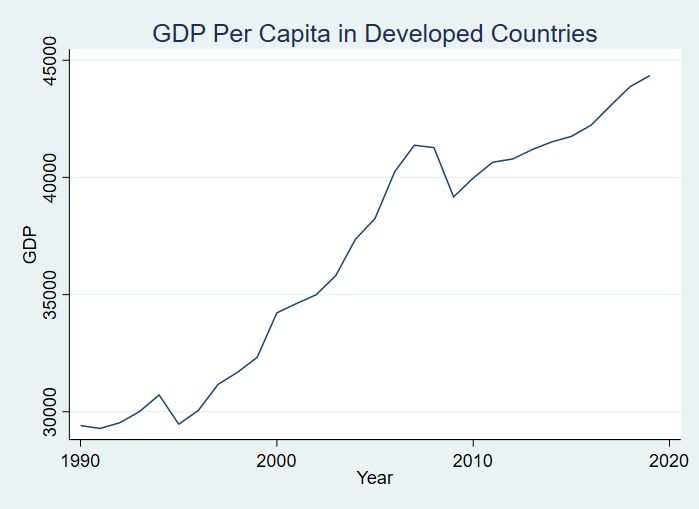
\includegraphics[width=0.5\linewidth]{FINAL FINAL GDP DEVELOPED.png}
    \caption{Enter Caption}
    \label{fig:enter-label}
\end{figure}
\begin{figure}
    \centering
    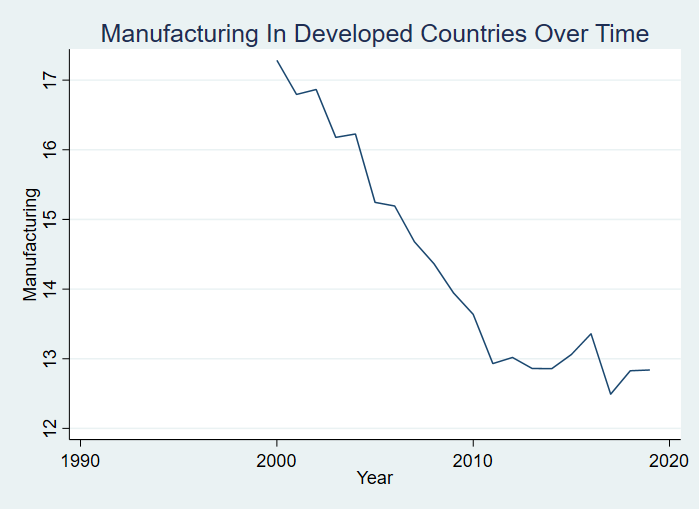
\includegraphics[width=0.5\linewidth]{FINAL FINAL MANU DEVELOPED.png}
    \caption{Enter Caption}
    \label{fig:enter-label}
\end{figure}


\subsection{Data Limitations}
This study relies on aggregate data, which may obscure important variations between individual countries. Furthermore, gaps in data reporting, especially in developing countries, could affect the validity of our results. Despite these limitations, the dataset provides valuable insights into long-term economic and industrial trends on a global scale.

\subsection{Exclusions and Clarifications}
Our analysis excludes data after 2019 to avoid the confounding effects of the COVID-19 pandemic, which introduced unprecedented disruptions to global economies and labor markets. Additionally, our focus on two primary variables, \textit{Manufacturing Employment Share} and \textit{GDP per Capita}, allows us to conduct a more detailed examination of their relationship across different stages of economic development.


\section{Results}
\label{sec:result}

The analysis evaluated the relationship between manufacturing employment and GDP per capita across developed and developing countries from 1990 to 2019. As manufacturing employment decreases, GDP increases, which indicates a negative relationship between manufacturing employment and GDP. The null hypothesis that goes along with our hypothesis is that there is no relationship between manufacturing employment and GDP. Descriptive statistics revealed distinct patterns between these two groups, reflecting their varying stages of industrialization and economic growth.

\subsection{Graphical Trends}

\begin{figure}
    \centering
    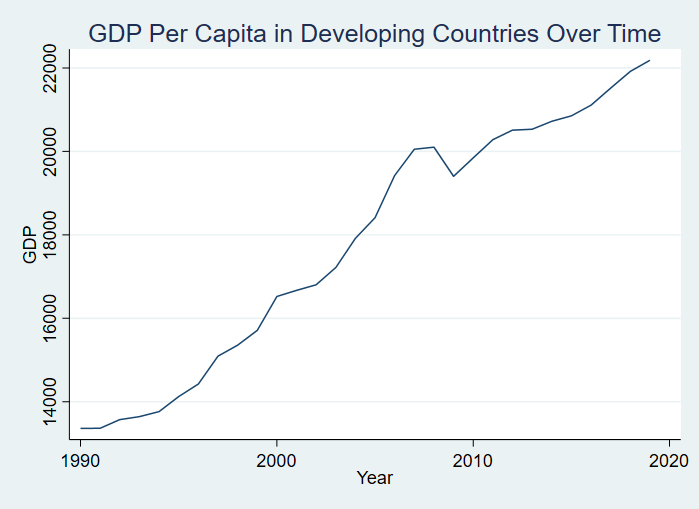
\includegraphics[width=0.5\linewidth]{GDP DEVELOPING GRAPH.png}
    \caption{GDP Per Capita Over Time}
    \label{fig:enter-label}
\end{figure}
\begin{figure}
    \centering
    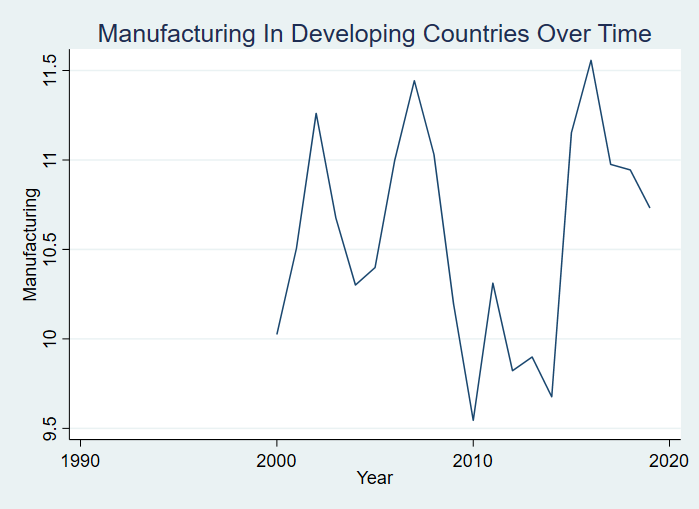
\includegraphics[width=0.5\linewidth]{FINAL GRAPH MFT DEVELOPING.png}
    \caption{Manufacturing Over Time}
    \label{fig:enter-label}
\end{figure}
\item Manufacturing employment shares exhibited fluctuations but generally declined after 2010. However, GDP per capita followed a steady upward trajectory, suggesting that factors beyond manufacturing, such as technological adoption or service sector expansion, are driving economic growth.


\begin{figure}
    \centering
    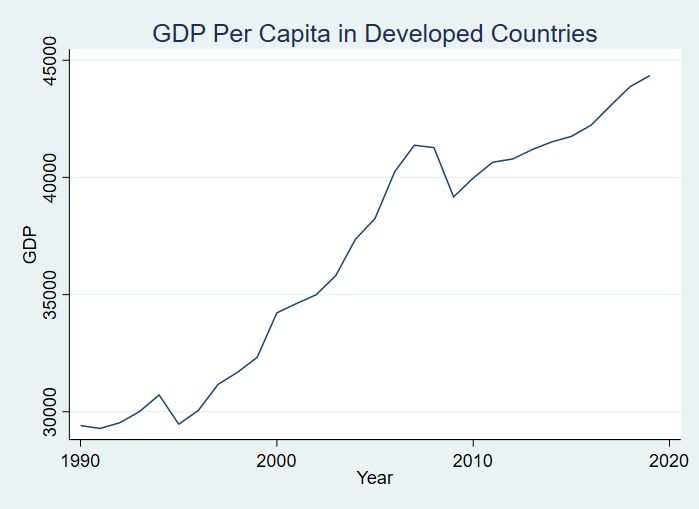
\includegraphics[width=0.5\linewidth]{FINAL FINAL GDP DEVELOPED.png}
    \caption{GDP Per Capita Over Time}
    \label{fig:enter-label}
\end{figure}
\begin{figure}
    \centering
    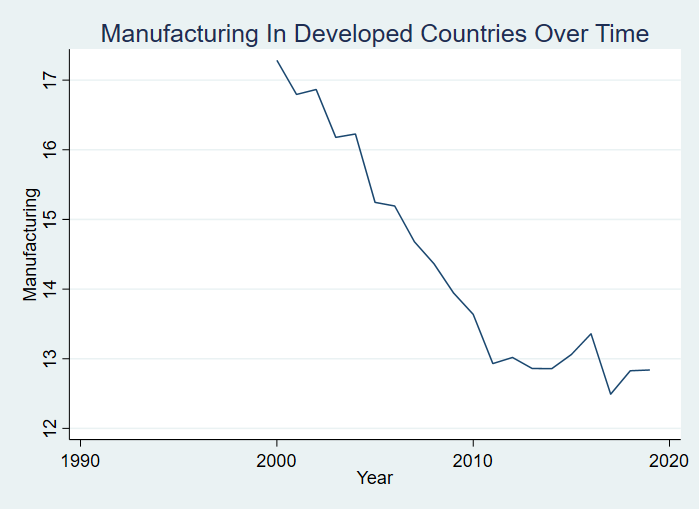
\includegraphics[width=0.5\linewidth]{FINAL FINAL MANU DEVELOPED.png}
    \caption{Manufacturing Over Time}
    \label{fig:enter-label}
\end{figure}


\section{Discussion}
\label{sec:discussion}


The analysis relies on aggregate data, which may mask important variations between countries. Further, many developing countries lack continuous data, with some years not reporting any numbers, causing sudden fluctuations in manufacturing data and its visual representation. On a similar note, the time frame for developed economies (2000–2019) and developing economies (1990–2019) varies, potentially affecting the consistency of the analysis.
In developed countries, the progressive switch to tertiary industries plays a significant role in GDP changes, as demonstrated by a relatively low R-squared.

Further research should monitor future changes, directly seeking out data from respective government and independent sources, and filling in blanks.


\section{Conclusion}
\label{sec:conclusion}

Manufacturing and economic growth are unequivocally linked. Previous literature has largely focused on the shift toward manufacturing across time, starting from the industrial revolution, and the income gaps that have risen across the world today.  We examined the relationship between manufacturing and GDP, and how this differs between developed and developing countries.

\newpage
\section*{Bibliography}
\singlespacing
\setlength\bibsep{0pt}

You can either explicitly include your list of references, or you can learn to use BibTex so that it includes the references automatically.

Either way, this list should include ONLY the papers (reports, book chatpers, etc.) that you actually cite in the text (no extra).

At the same time EVERYTHING you cite in the main text must have an entry here (no references in text that don't have something here).

You can choose which citation style to follow. Whichever you choose, you must follow it consistently.

\newpage
\section*{Data Appendix} \label{sec:appendixa}
\addcontentsline{toc}{section}{Appendix A}

Once the data is categorized, we manually selected all countries, then click on the download, clicking on the "Data" option before downloading the data set completely. 

\end{document}
